\documentclass[11pt,a4paper]{article}

\usepackage[utf8]{inputenc}
\usepackage[T1]{fontenc}
\usepackage{lmodern}
\usepackage{microtype}
\usepackage{amsmath,amssymb,amsfonts}
\usepackage{booktabs}
\usepackage{tabularx}
\usepackage{multirow}
\usepackage{caption}
\usepackage{float}
\usepackage{graphicx}
\usepackage{setspace}
\usepackage{enumitem}
\usepackage{parskip}
\usepackage{array}
\usepackage{dcolumn}
\usepackage{datetime}

\usepackage{tabularx}
\usepackage{adjustbox}

\usepackage[sc]{mathpazo}
\usepackage[scaled=0.95]{helvet}
\usepackage{courier}
\linespread{1.08}

\usepackage{xcolor}
\definecolor{navyblue}{rgb}{0,0,0.7}

\usepackage[
  a4paper,
  top=2.5cm, bottom=2.8cm,
  left=2.8cm, right=2.8cm,
  headheight=14pt
]{geometry}

\usepackage{fancyhdr}
\pagestyle{fancy}
\fancyhf{}
\renewcommand{\headrulewidth}{0pt}
\fancyfoot[C]{\small\thepage}

\usepackage{titlesec}

\titleformat{\section}
  {\normalfont\large\bfseries\scshape}{\thesection.}{0.6em}{}
\titleformat{\subsection}
  {\normalfont\normalsize\bfseries}{\thesubsection}{0.5em}{}
\titleformat{\subsubsection}
  {\normalfont\normalsize\itshape}{\thesubsubsection}{0.5em}{}
\titleformat{\paragraph}[runin]
  {\normalfont\normalsize\bfseries}{}{0em}{}[.\enspace]

\titlespacing*{\section}      {0pt}{18pt}{8pt}
\titlespacing*{\subsection}   {0pt}{12pt}{4pt}
\titlespacing*{\subsubsection}{0pt}{8pt}{2pt}

\usepackage[font=small,labelfont=bf,labelsep=period,
            justification=justified,skip=6pt]{caption}

\usepackage{hyperref}
\hypersetup{
  colorlinks=true, linkcolor=black, anchorcolor=black,
  citecolor=navyblue, filecolor=black, menucolor=black,
  runcolor=black, urlcolor=black,
  pdfauthor={Yvan Landry Ndzonde Fonkou},
  pdftitle={Do Nonparametric and Linear Methods Agree?},
  pdfsubject={Methodological Comparison, Causal Discovery, Finance},
  pdfkeywords={tMIIC, Granger causality, VECM, conditional dependence,
               sector ETFs, nonparametric, cointegration}
}

\usepackage[authoryear,round,sort]{natbib}
\bibpunct{(}{)}{;}{a}{,}{,}
\setlength{\bibsep}{4pt}

\newcolumntype{d}[1]{D{.}{.}{#1}}
\newdateformat{monthyear}{\monthname[\THEMONTH]\ \THEYEAR}

% ── Title block ───────────────────────────────────────────
\title{%
  \vspace{-0.5cm}
  {\large\bfseries
    Dollar-Cost Averaging Versus Lump-Sum-Investing: Evidence from France }
}

\author{%
  Yvan Landry Ndzonde Fonkou\\[2pt]
  \small Independent Researcher\\
  \small \href{mailto:yvanndzonde@gmail.com}{yvanndzonde@gmail.com}
}

\date{\small\monthyear\today}

% ═══════════════════════════════════════════════════════════
\begin{document}
\maketitle
\thispagestyle{fancy}
\vspace{-4pt}

% ── Abstract ──────────────────────────────────────────────
\begin{abstract}
\end{abstract}

% ═══════════════════════════════════════════════════════════
\section{Introduction}
\label{sec:intro}
% ═══════════════════════════════════════════════════════════
Dollar-Cost Averaging (DCA) is an investment strategy whereby an investor allocates capital in equal amounts at regular intervals over a predefined investment horizon. This progressive investment mechanism is generally motivated by its ability to reduce timing risk, particularly the risk of committing a large amount of capital at market peaks. By construction, DCA leads investors to purchase more shares when prices are low and fewer when prices are high, thereby smoothing the average purchase cost over time \citep{dichtl2011}. From a theoretical perspective, DCA can also be interpreted as a risk management device, acting as a partial hedge against short-term market volatility by spreading entry points across time \citep{milevsky2003}.

In contrast, Lump-Sum Investing (LSI) consists of investing the entire available capital at a single point in time, thus providing immediate and full exposure to market risk. In upward-trending markets, this strategy is often expected to outperform DCA, as capital is deployed earlier and benefits more rapidly from market appreciation. Consequently, LSI may appear more attractive to investors with strong bullish expectations. Conversely, DCA tends to be preferred in environments characterized by heightened uncertainty or anticipated downturns \citep{grable2015}. However, such preferences implicitly rely on the ability to time market conditions, which remains notoriously difficult in practice.

This tension naturally raises a fundamental question for investors: which strategy should be preferred when entering financial markets under uncertainty? More specifically, beyond conditional preferences based on market expectations, it becomes essential to assess which approach delivers superior performance on average, and how sensitive this performance is to the timing of market entry.

The objective of this study is therefore to provide a comparative analysis of DCA and LSI strategies. In particular, we aim to contribute to the existing literature by offering new empirical evidence based on the French market. Additionally, this work seeks to enrich the debate by linking investment outcomes to behavioral considerations, thereby providing a more comprehensive understanding of how investors navigate the trade-off between risk and return when choosing between these two widely used investment strategies.


\section{Methodology}

\subsection{Investment Framework and Assumptions}

This study compares the performance of Dollar-Cost Averaging (DCA) and
Lump-Sum Investing (LSI) on the French equity market. Both strategies are
evaluated under a common set of assumptions, consistent with the existing
literature (Leggio and Lien, 2001; Eriksson and Fransson, 2021).

An investor is assumed to have a fixed initial capital $W_0$ available at
time $t = 0$. This capital represents a lump sum that could, in principle,
be deployed immediately or phased into the market over a predefined horizon. The investor selects a single stock listed on Euronext Paris and commits to one of the two strategies without any subsequent tactical
reallocation. No transaction costs are considered. Dividends are reinvested continuously through an explicit dividend-reinvestment mechanism (Section~2.2--2.3), applied to raw, non-dividend-adjusted price series so that each distribution is credited exactly once.\footnote{Total-return data providers already fold historical dividends into the price series; combining such a series with an explicit reinvestment rule would double-count every distribution.} Returns are expressed in nominal terms, with no adjustment for inflation. Cash awaiting deployment under DCA is remunerated at the historical rate of the \emph{Livret A}, the standard capital-guaranteed savings account available to French retail investors, compounded daily on a calendar-day basis.\footnote{Rate schedule (Banque de France): 1.25\% (2009--2010), rising to 2.25\% (2011--2013), then declining to 0.75\% (2015--2020).} This is a more realistic assumption than crediting no return at all, and reflects the natural opportunity cost of idle cash for a retail investor, as opposed to an interbank rate that such an investor cannot access.

\subsection{Lump Sum Investing (LSI)}

Under the Lump Sum Investing (LSI) strategy, the entire initial capital $W_0$ is fully deployed at the inception of the investment horizon $t_0$.  At the effective start date $t_0$, shares are acquired at the observed market opening price $P_{\text{open}}(t_0)$. Fractional shares are fully preserved without rounding or residual cash drag, yielding an initial share count $N_{\text{LSI}}(t_0)$:
\begin{equation}
N_{\text{LSI}}(t_0) = \frac{W_0}{P_{\text{open}}(t_0)}
\end{equation}

The dividend paid during the holding periods are fully reinvested using the dividend reinvestment plan (DRIP). Let $\mathcal{D} = \{t \in (t_0, t_F] \mid D_t > 0\}$ be the set of discrete dates within the investment window where a cash dividend per share $D_t$ is distributed. On any dividend ex-date $t \in \mathcal{D}$, the accumulated cash payload is immediately converted into additional fractional shares at the daily market closing price $P_{\text{close}}(t)$. The share tracking engine updates iteratively:
\begin{equation}
N_{\text{LSI}}(t) = N_{\text{LSI}}(t^-) + \frac{N_{\text{LSI}}(t^-) \times D_t}{P_{\text{close}}(t)}
\end{equation}
where $N_{\text{LSI}}(t^-)$ represents the share inventory held immediately prior to the dividend distribution at time $t$. The daily mark-to-market value of the portfolio, or equity curve $V_{\text{LSI}}(t)$, is calculated across the entire timeline by scaling the share balance held \emph{at each date} against that date's closing price:
\begin{equation}
V_{\text{LSI}}(t) = N_{\text{LSI}}(t) \times P_{\text{close}}(t), \quad \forall t \in [t_0, t_F]
\end{equation}

\subsection{Dollar-Cost Averaging (DCA)}

Under the Dollar-Cost Averaging (DCA) strategy, the initial capital $W_0$ is structured into systematic tranches to mitigate timing risk rather than being deployed as a single lump sum.

Let $\mathcal{T}_{\text{theory}}$ be the set of theoretical investment dates generated by the user-defined frequency $\text{freq} \in \{\text{D, W, M, Q, S, A}\}$. Because theoretical dates can fall on weekends or market holidays, the execution engine maps each theoretical date to the first available active trading session on or after it. This yields an ordered set of $N$ actual trading dates:
\begin{equation}
\mathcal{T} = \{t_1, t_2, \dots, t_N\} \subseteq [t_0, t_F]
\end{equation}
The total capital $W_0$ is divided into $N$ equal allocations, determining a static cash tranche size $W_{\text{tranche}}$:
\begin{equation}
W_{\text{tranche}} = \frac{W_0}{N}
\end{equation}

At each scheduled investment date $t_k \in \mathcal{T}$, the static tranche $W_{\text{tranche}}$ is used to purchase additional asset fractions at the observed market opening price $P_{\text{open}}(t_k)$. Concurrently, the engine tracks discrete dividend distributions. Let $\mathcal{D} = \{t \in (t_0, t_F] \mid D_t > 0\}$ be the set of active dividend ex-dates.

The physical share inventory $N_{\text{DCA}}(t)$ updates sequentially for every chronological market date $t \in [t_0, t_F]$ according to the following cumulative matching logic:
\begin{equation}
N_{\text{DCA}}(t) = N_{\text{DCA}}(t^-) + \Delta N_{\text{tranche}}(t) + \Delta N_{\text{DRIP}}(t)
\end{equation}
where $N_{\text{DCA}}(t^-)$ is the share balance from the prior trading day, and the incremental additions are defined as:
\begin{equation}
\Delta N_{\text{tranche}}(t) = \begin{cases}
\dfrac{W_{\text{tranche}}}{P_{\text{open}}(t)} & \text{if } t \in \mathcal{T} \\
0 & \text{otherwise}
\end{cases}
\end{equation}

\begin{equation}
\Delta N_{\text{DRIP}}(t) = \begin{cases}
\dfrac{N_{\text{DCA}}(t^-) \times D_t}{P_{\text{close}}(t)} & \text{if } t \in \mathcal{D} \text{ and } N_{\text{DCA}}(t^-) > 0 \\
0 & \text{otherwise}
\end{cases}
\end{equation}

Capital not yet deployed is held as cash $C(t)$, remunerated at the annualized Livret~A rate $r(t)$ (Section~2.1), compounded on the number of calendar days $\Delta_t$ elapsed since the previous trading session and debited by each tranche as it is invested:
\begin{equation}
C(t) = C(t^-) \times \big(1 + r(t)\big)^{\Delta_t / 365} - W_{\text{tranche}} \cdot \mathbb{1}\{t \in \mathcal{T}\}, \qquad C(t_0) = W_0
\end{equation}
The daily mark-to-market equity curve $V_{\text{DCA}}(t)$ therefore tracks both the growing share position and the residual cash balance:
\begin{equation}
V_{\text{DCA}}(t) = N_{\text{DCA}}(t) \times P_{\text{close}}(t) + C(t), \quad \forall t \in [t_0, t_F]
\end{equation}

\subsection{Rolling Window Simulation and performance metric}

Rather than evaluating the strategies over a single fixed period, this study employs a multi-layered rolling window approach, consistent with the methodology of Leggio and Lien (2001) and Eriksson and Fransson (2021).

Formally, let $t_{\text{start}}$ be the baseline historical anchor date. For a fixed investment horizon $H = 5$ years and an execution step size $\Delta m = \text{shift\_months}$, the sequence of chronological window start dates $\{t_0^{(i)}\}_{i=1}^M$ and corresponding terminal boundaries $\{t_F^{(i)}\}_{i=1}^M$ are mapped sequentially via the index $i \in \{1, 2, \dots, M\}$:
\begin{equation}
t_0^{(i)} = t_{\text{start}} + (i - 1) \times \Delta m, \quad t_F^{(i)} = t_0^{(i)} + H
\end{equation}
where $M$ denotes the user-defined total number of independent rolling horizons. For each localized window $i$, the engine runs two isolated, path-dependent physical atomic simulations to resolve the underlying asset vectors and extract a clean cross-sectional matrix of three core performance structures:

\textbf{Performance Measures}

Extracted directly by evaluating the terminal mark-to-market capital yield against the localized initial deployment $W_0$:
\begin{equation}
\text{HPR}_{\text{strat}}^{(i)} = \frac{V_{\text{strat}}^{(i)}\big(t_F^{(i)}\big) - W_0}{W_0}, \quad \text{strat} \in \{\text{LSI, DCA}\}
\end{equation}
The cross-strategy alpha differential for each rolling iteration is recorded directly into the temporal tracking series as:
\begin{equation}
\Delta\text{HPR}^{(i)} = \text{HPR}_{\text{LSI}}^{(i)} - \text{HPR}_{\text{DCA}}^{(i)}
\end{equation}

Let $r_t^{(i)} = \ln\big(V_{\text{strat}}^{(i)}(t) / V_{\text{strat}}^{(i)}(t-1)\big)$ define the daily log return vector on active trading sessions inside window $i$. Given an annualized risk-free benchmark $r_f$, the daily excess asset return series is structured as $r_{e,t}^{(i)} = r_t^{(i)} - \frac{r_f}{252}$. The annualized Sharpe ($\mathcal{S}_h^{(i)}$) and Sortino ($\mathcal{S}_o^{(i)}$) profiles are modeled via standard sample variance and localized downside semi-variance frameworks:
\begin{equation}
\mathcal{S}_h^{(i)} = \sqrt{252} \times \frac{\mathbb{E}\big[r_{e,t}^{(i)}\big]}{\sigma\big(r_{e,t}^{(i)}\big)}
\end{equation}
\begin{equation}
\mathcal{S}_o^{(i)} = \sqrt{252} \times \frac{\mathbb{E}\big[r_{e,t}^{(i)}\big]}{\sigma_{\text{down}}\big(r_{e,t}^{(i)}\big)}, \quad \text{where } \sigma_{\text{down}}\big(r_{e,t}^{(i)}\big) = \sqrt{\frac{1}{K-1}\sum_{t \in \text{neg}} \Big(r_{e,t}^{(i)} - \mathbb{E}\big[r_{e,t}^{(i)}\big]\Big)^2}
\end{equation}
where $\text{neg} = \{t \mid r_{e,t}^{(i)} < 0\}$ represents the subset of trading days with negative excess performance, and $K = |\text{neg}|$.

To evaluate structural paths across business cycles (expansions, contractions, and market crises), each window is tagged with its baseline entry price level $P_{\text{open}}(t_0^{(i)})$. This acts as an exogenous conditioning variable used to map how the performance gap $\Delta\text{HPR}^{(i)}$ behaves across varying asset price regimes.

\subsection{Statistical Framework and Hypothesis Testing}

To rigorously assess whether the performance differences between the LSI and DCA strategies are statistically meaningful or merely artifacts of sample volatility, we implement a structured inferential framework. Given that our rolling window simulation evaluates both strategies over the exact same cross-sectional market paths within each window $i$, the resulting performance vectors are intrinsically paired.

\subsubsection{Normality and Specification Diagnostics}

Prior to conducting parametric inference, the distributional properties of the performance differentials $\Delta\text{HPR}^{(i)}$ are formally evaluated to verify the underlying assumptions of ordinary least squares and classical standard errors. We apply the Shapiro-Wilk test for normality, which computes the test statistic $W$:
\begin{equation}
W = \frac{\left(\sum_{i=1}^M a_i \Delta\text{HPR}^{(i)}\right)^2}{\sum_{i=1}^M \left(\Delta\text{HPR}^{(i)} - \overline{\Delta\text{HPR}}\right)^2}
\end{equation}
where $a_i$ represents the weights derived from the covariances of the order statistics of a standard normal distribution, and $\overline{\Delta\text{HPR}}$ is the sample mean differential. Under the null hypothesis $H_0^{\text{SW}}$, the differences are normally distributed. If $H_0^{\text{SW}}$ is rejected at a significance level of $\alpha = 0.05$, non-parametric alternatives (such as the Wilcoxon Signed-Rank test) are reported to complement the parametric inference.

\subsubsection{Paired Student's t-Test}

Subject to satisfactory specification diagnostics, a two-sided paired Student's $t$-test is deployed to test the null hypothesis that the true mean performance differential between LSI and DCA is equal to zero, against the alternative hypothesis that their expected returns diverge:
\begin{equation}
\begin{cases}
H_0: \mu_{\Delta\text{HPR}} = 0 \\
H_1: \mu_{\Delta\text{HPR}} \neq 0
\end{cases}
\end{equation}

By accounting for the path-dependent covariance common to both strategies within each simulation window, the paired $t$-statistic eliminates the cross-sectional variance drag, optimizing statistical power. The test statistic $t$ is formulated as:
\begin{equation}
t = \frac{\overline{\Delta\text{HPR}}}{s_{\Delta} / \sqrt{M}}
\end{equation}
where $s_{\Delta}$ represents the sample standard deviation of the paired differences, defined as:
\begin{equation}
s_{\Delta} = \sqrt{\frac{1}{M-1} \sum_{i=1}^M \left(\Delta\text{HPR}^{(i)} - \overline{\Delta\text{HPR}}\right)^2}
\end{equation}

The computed statistic follows a Student's $t$-distribution with $M - 1$ degrees of freedom. To determine the directionality of the outperformance under a stricter framework, we also compute one-sided upper tail $p$-values testing $H_0: \mu_{\Delta\text{HPR}} \leq 0$ against $H_1: \mu_{\Delta\text{HPR}} > 0$ to formally isolate the statistical significance of the LSI premium.

\section{Results}

\subsection{Cross-Sectional Analysis on the Aggregate CAC 40 Index}

Rolling window simulations over the period starting in 2010 indicate a structural dominance of the Lump-Sum Investing (LSI) strategy over Dollar-Cost Averaging (DCA). The only tactical horizons where DCA marginally outperforms LSI correspond to entry dates spanning from early 2010 to late 2011.

\begin{figure}[H]
    \centering
    \includegraphics[width=0.85\linewidth]{image2.png}
    \caption{Temporal evolution of LSI vs. Monthly DCA HPR across rolling 5-year horizons (2010--2015).}
    \label{fig:cac40_temporal_scatter}
\end{figure}
This specific outperformance window is fundamentally linked to the macroeconomic regime of the French equity market at that time. Following the 2008 financial crisis and structural shocks from the Eurozone sovereign debt crisis (notably the Greek default risks), the CAC 40 experienced high volatility and a prolonged sideways-to-negative trend. In such non-directional or declining markets, DCA mechanically mitigates timing risk by acquiring cheaper fractions of shares, lowering the average cost basis. Conversely, as soon as the index enters a sustained secular bull regime post-2012, LSI captures the full upward beta from day one, exposing the cash drag inherent to DCA.

\begin{figure}[H]
    \centering
    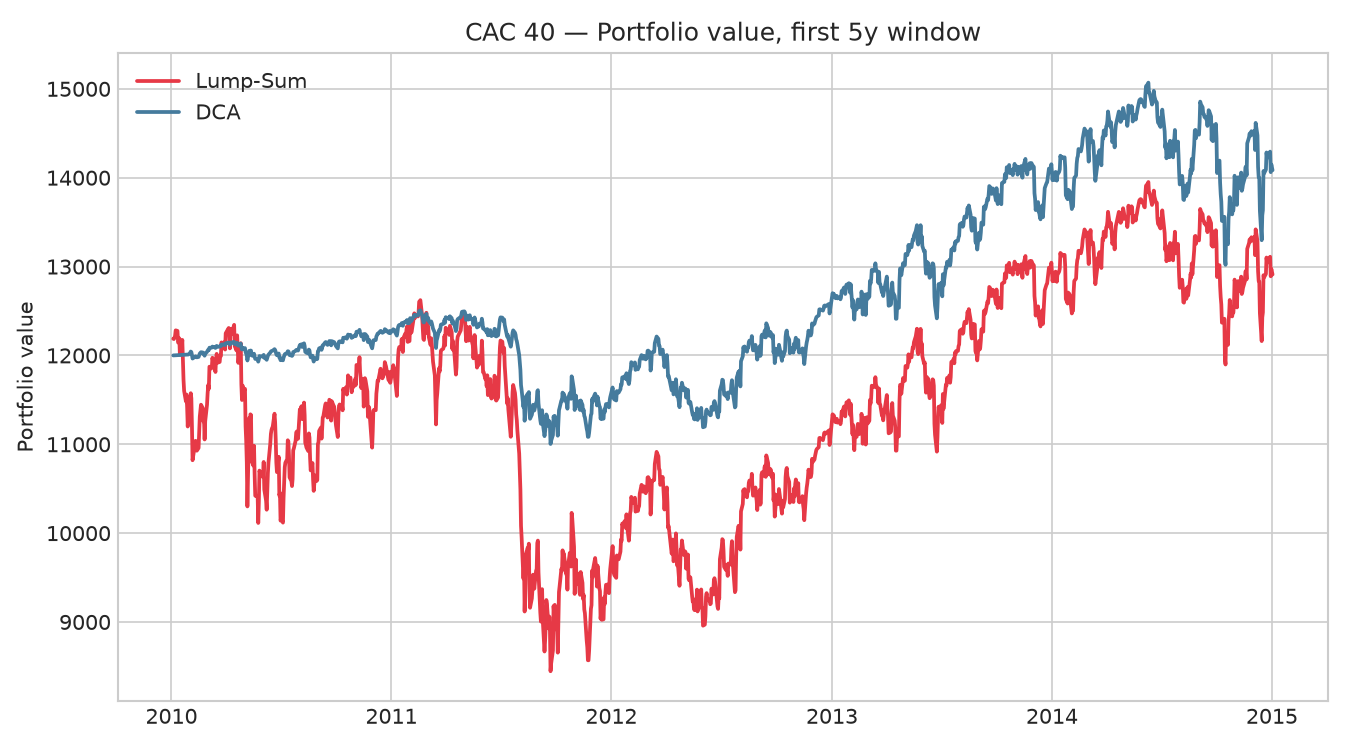
\includegraphics[width=0.8\linewidth]{equity_curves.png}
    \caption{Portfolio value over time, LSI vs.\ semi-annual DCA, CAC~40 index, illustrative 5-year window (2010--01 to 2012--01).}
    \label{fig:equity-curves}
\end{figure}

\subsubsection{Sensitivity Analysis to DCA Infusion Frequency}

Table~\ref{tab:dca_frequency} provides a comparative analysis of alternative DCA scheduling regimes (Monthly, Semi-Annual, and Annual) against the baseline LSI.

\begin{table}[htbp]
\centering
\caption{CAC 40 Index Backtest Framework Summary ($\Delta t = 5$ Years, $M = 60$ Windows, $W_0 = \text{\euro{12,000}}$).}
\label{tab:dca_frequency}
\small
\begin{tabular}{llccccc}
\hline
\textbf{DCA Frequency} & \textbf{Metric} & \textbf{LSI Mean} & \textbf{LSI Std} & \textbf{DCA Mean} & \textbf{DCA Std} & \textbf{LSI Wins (\%)} \\ \hline
\textbf{Monthly} & HPR (\%) & 33.11 & 16.46 & 19.63 & 7.93 & 76.67 \\
(12$\times$/year) & CAGR (\%) & 5.76 & 2.60 & 3.62 & 1.36 & 76.67 \\
 & $W_{\text{final}}$ (\euro{}) & 15,973.62 & 1,975.59 & 14,355.45 & 951.68 & 76.67 \\ \hline
\textbf{Semi-Annual} & HPR (\%) & 33.11 & 16.46 & 20.76 & 8.27 & 73.33 \\
(2$\times$/year) & CAGR (\%) & 5.76 & 2.60 & 3.81 & 1.41 & 73.33 \\
 & $W_{\text{final}}$ (\euro{}) & 15,973.62 & 1,975.59 & 14,491.58 & 991.96 & 73.33 \\ \hline
\textbf{Annual} & HPR (\%) & 33.11 & 16.46 & 20.89 & 7.42 & 73.33 \\
(1$\times$/year) & CAGR (\%) & 5.76 & 2.60 & 3.84 & 1.26 & 73.33 \\
 & $W_{\text{final}}$ (\euro{}) & 15,973.62 & 1,975.59 & 14,506.40 & 890.70 & 73.33 \\ \hline
\end{tabular}
\end{table}

Lowering the DCA sampling frequency front-loads larger tranches earlier in the window: mean HPR rises from 19.63\% (monthly) to 20.76\% (semi-annual) and 20.89\% (annual), with rapidly diminishing increments as the tranche count falls further. Across all configurations, LSI wins 73--77\% of rolling windows, delivering higher expected returns at the cost of markedly higher variance ($\sigma_{\text{LSI}} \approx 16.5\%$ vs.\ $\sigma_{\text{DCA}} \approx 7.4$--$8.3\%$).

\subsection{Cross-Sectional Granular Analysis across CAC 40 Individual Stocks}

The cross-sectional analysis across individual constituents of the CAC 40 confirms that the outperformance of Lump-Sum Investing (LSI) observed at the aggregate index level remains highly robust when broken down by individual stock tickers.

\begin{table}[H]
\centering
\caption{Cross-Sectional Sector Analysis: Lump-Sum Investing (LSI) vs. Semi-Annual DCA on CAC
40 Components (M = 60 Rolling Windows)}
\label{tab:lsi_vs_dca_sectors}
\small
\begin{tabularx}{\textwidth}{X c c c c c}
\hline
 & \multicolumn{2}{c}{\textbf{Lump-Sum Investing (LSI)}} & \multicolumn{2}{c}{\textbf{Semi-Annual DCA (2$\times$/year)}} & \textbf{LSI Win} \\
\cline{2-5}
\textbf{Company} & \textbf{HPR (\%)} & \textbf{Std} & \textbf{HPR (\%)} & \textbf{Std} & \textbf{Rate (\%)} \\
\hline
Capgemini & 173 & 58 & 84 & 33 & 98 \\
Michelin & 90 & 40 & 44 & 19 & 100 \\
Renault & 113 & 78 & 48 & 48 & 100 \\
Stellantis & 241 & 141 & 115 & 53 & 87 \\
Schneider Electric & 48 & 29 & 26 & 13 & 90 \\
Crédit Agricole & 93 & 107 & 52 & 31 & 67 \\
BNP Paribas & 47 & 52 & 26 & 22 & 67 \\
AXA & 107 & 53 & 52 & 27 & 93 \\
Société Générale & 47 & 76 & 25 & 31 & 60 \\
Air Liquide & 57 & 17 & 31 & 12 & 100 \\
Vinci & 121 & 42 & 64 & 14 & 98 \\
Engie & $-2$ & 16 & 5 & 10 & 32 \\
Orange & 70 & 36 & 43 & 19 & 63 \\
TotalEnergies & 50 & 18 & 28 & 8 & 95 \\
Veolia & 92 & 62 & 59 & 26 & 67 \\
EssilorLuxottica & 91 & 39 & 41 & 23 & 100 \\
Sanofi & 56 & 40 & 24 & 21 & 97 \\
Eurofins Scientific & 382 & 229 & 129 & 76 & 100 \\
Airbus & 195 & 59 & 85 & 23 & 100 \\
Alstom & 13 & 39 & 20 & 23 & 32 \\
Thales & 205 & 71 & 99 & 32 & 97 \\
Safran & 201 & 49 & 90 & 21 & 100 \\
Legrand & 106 & 38 & 49 & 19 & 100 \\
Saint-Gobain & 34 & 35 & 19 & 19 & 75 \\
Christian Dior & 151 & 58 & 83 & 36 & 100 \\
Kering & 161 & 83 & 97 & 60 & 100 \\
LVMH & 107 & 50 & 63 & 31 & 100 \\
L'Oréal & 108 & 23 & 53 & 14 & 100 \\
Hermès & 130 & 51 & 62 & 14 & 97 \\
Accor & 58 & 32 & 30 & 23 & 92 \\
Danone & 50 & 12 & 28 & 8 & 100 \\
Carrefour & 0 & 32 & 3 & 24 & 42 \\
Pernod Ricard & 75 & 20 & 41 & 12 & 100 \\
Bouygues & 75 & 52 & 44 & 21 & 68 \\
Publicis Groupe & 55 & 54 & 19 & 29 & 90 \\
Teleperformance & 344 & 120 & 153 & 26 & 100 \\
Vivendi & 170 & 34 & 81 & 18 & 100 \\
Dassault Systèmes & 163 & 27 & 78 & 16 & 100 \\
\hline
\end{tabularx}
\end{table}


Across nearly all companies evaluated, LSI delivers a substantially higher mean Holding Period Return (HPR) compared to the Semi-Annual DCA strategy, capturing a systematic premium from immediate market exposure. High-growth or volatile assets such as Eurofins Scientific, Teleperformance, and Vivendi display the most dramatic absolute performance gaps, where LSI leverages compound returns on early capital commitment.

Concurrently, the empirical evidence illustrates the classic risk-return trade-off: the higher expected returns of LSI are systematically accompanied by an elevated standard deviation across all assets. In contrast, the Semi-Annual DCA effectively acts as a volatility smoothing mechanism, significantly compressing the standard deviation of terminal outcomes.

Nevertheless, this variance reduction comes at a steep opportunity cost for most names. LSI maintains a dominant win rate, reaching 100\% for the majority of individual stocks. The structural exceptions, where DCA outright outperforms on a majority of windows, are Engie (LSI win rate of 32\%), Alstom (32\%), and Carrefour (42\%) --- all three range-bound or declining over large stretches of the sample period --- with Société Générale (60\%) and Orange (63\%) forming a second, more moderate tier. This confirms that DCA's relative value is strictly conditional on non-bullish underlying regimes.

\begin{figure}[H]
    \centering
    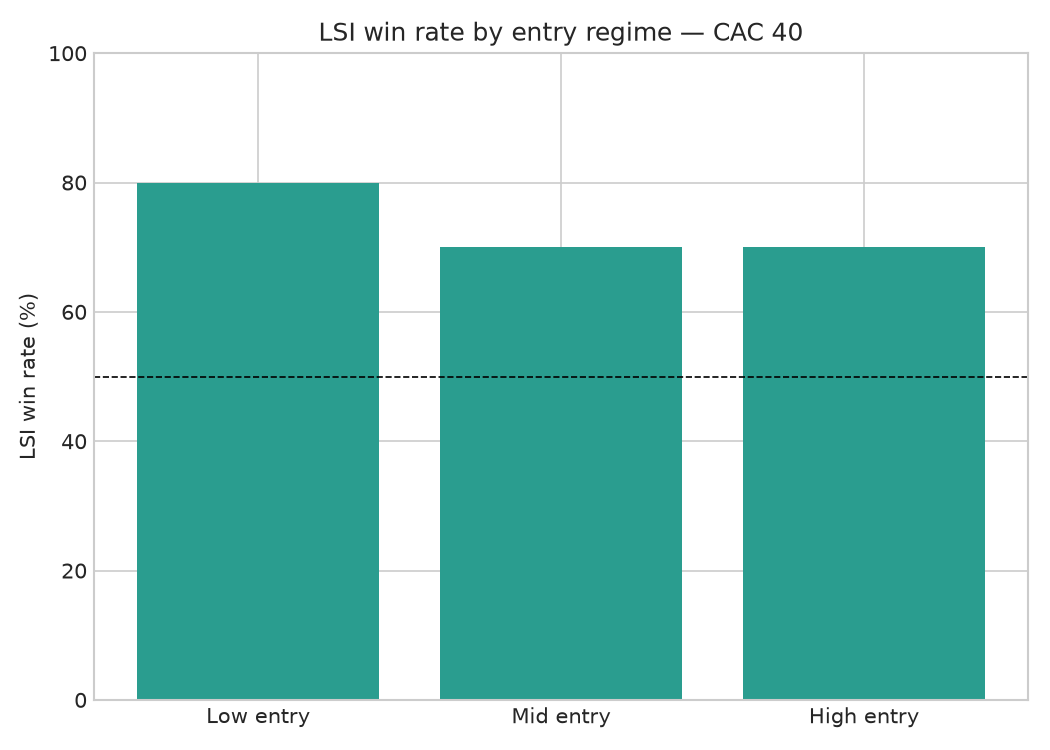
\includegraphics[width=0.75\linewidth]{win_rate_by_regime.png}
    \caption{LSI win rate by entry-market regime (CAC~40 index, tertiles of entry price level).}
    \label{fig:win-rate-regime}
\end{figure}


\begin{thebibliography}{99}
\setlength{\itemsep}{3pt}

\bibitem[Dichtl and Drobetz(2011)]{dichtl2011}
Dichtl, H. and Drobetz, W. (2011).
Dollar-Cost Averaging and Prospect Theory Investors: An Explanation for a Popular Investment Strategy.
\textit{Journal of Behavioral Finance}, 12(1), 41--52.

\bibitem[Milevsky and Posner(2003)]{milevsky2003}
Milevsky, M. A. and Posner, S. E. (2003).
A continuous-time reexamination of dollar-cost averaging.
\textit{International Journal of Theoretical and Applied Finance}, 6(1), 173--194.

\bibitem[Grable and Chatterjee(2015)]{grable2015}
Grable, J. E. and Chatterjee, S. (2015).
Another look at lump-sum versus dollar-cost averaging.
\textit{Journal of Financial Service Professionals}, 69(5), 16--18.

\end{thebibliography}

\end{document}
